\documentclass[11pt,a4paper,oneside]{report}

% Load Preamble and Macros
% ==============================================================================
% SocialMirror-AI Preparatory Report - Preamble (Hebrew & English Multilingual)
% University of Haifa - AI Agents Course (Assignment 2)
% ==============================================================================

% Page Geometry & Margins
\usepackage{geometry}
\geometry{
    a4paper,
    top=2.5cm,
    bottom=2.5cm,
    left=2.8cm,
    right=2.8cm,
    headheight=20pt
}

\usepackage{setspace}
\onehalfspacing % 1.5 Line Spacing for Academic Readability

% Mathematics & Equations (Rendered in Standard LTR Math Mode)
\usepackage{amsmath}
\usepackage{amssymb}
\usepackage{amsfonts}
\usepackage{mathtools}

% Graphics & Tables
\usepackage{graphicx}
\usepackage{float}
\usepackage{booktabs}
\usepackage{tabularx}
\usepackage{multirow}
\usepackage{array}
\usepackage{environ}

% Colors & Themes
\usepackage[dvipsnames, table]{xcolor}
\definecolor{NavyBlueDark}{RGB}{10, 40, 95}
\definecolor{AccentTeal}{RGB}{0, 128, 128}
\definecolor{AccentCyan}{RGB}{0, 168, 204}
\definecolor{SlateGray}{RGB}{80, 90, 100}
\definecolor{SilverAccent}{RGB}{218, 224, 233}
\definecolor{LightBoxBg}{RGB}{245, 247, 250}
\definecolor{LightBlueBg}{RGB}{238, 244, 252}
\definecolor{BorderGray}{RGB}{200, 210, 225}
\definecolor{BrickRed}{RGB}{180, 40, 40}

% TikZ Vector Graphics
\usepackage{tikz}
\usetikzlibrary{shapes.geometric, arrows.meta, positioning, shadows, fit, backgrounds, calc}

% Captions Formatting
\usepackage{caption}
\usepackage{subcaption}
\captionsetup{font=small, labelfont=bf, margin=10pt}

% Hyperref & Navigation (Loaded BEFORE polyglossia so bidi handles RTL links properly)
\usepackage{hyperref}
\hypersetup{
    colorlinks=true,
    linkcolor=NavyBlueDark,
    citecolor=ForestGreen,
    filecolor=magenta,
    urlcolor=MidnightBlue,
    pdfstartview={FitH},
    pdfauthor={Shams Sabbagh and Malak},
    pdftitle={SocialMirror-AI: דוח הכנה אקדמי לפרויקט מחקר},
    pdfsubject={AI Agents - University of Haifa},
    plainpages=false,
    pdfpagelabels=true
}

% Font & Multilingual Support for XeLaTeX
\usepackage{fontspec}
\usepackage{polyglossia}
\setmainlanguage{hebrew}
\setotherlanguage{english}

% Hebrew and English Fonts (Standard Windows TrueType/OpenType Fonts)
\newfontfamily\hebrewfont{Arial}[Script=Hebrew]
\newfontfamily\hebrewfontsf{Arial}[Script=Hebrew]
\newfontfamily\hebrewfonttt{Courier New}[Script=Hebrew]
\newfontfamily\englishfont{Arial}

% Keep Hebrew heading for Bibliography even in English environment
\addto\captionsenglish{\renewcommand{\bibname}{\texthebrew{ביבליוגרפיה}}}

% Running Headers & Footers
\usepackage{fancyhdr}
\pagestyle{fancy}
\fancyhf{}
\fancyhead[R]{\small\nouppercase{\leftmark}}
\fancyhead[L]{\small\textenglish{\textsc{SocialMirror-AI}}}
\fancyfoot[C]{\thepage}
\renewcommand{\headrulewidth}{0.4pt}
\renewcommand{\footrulewidth}{0pt}

% Master Academic Editorial Styling for Headings
\makeatletter
\def\@makechapterhead#1{%
  \vspace*{10\p@}%
  {\parindent \z@ \raggedright \normalfont
    \ifnum \c@secnumdepth >\m@ne
        {\Large\bfseries\color{AccentTeal} \@chapapp\space \thechapter}
        \par\nobreak
        \vskip 6\p@
    \fi
    \interlinepenalty\@M
    {\Huge \bfseries \color{NavyBlueDark} #1\par\nobreak}
    \vskip 6\p@
    {\color{AccentCyan}\rule{\linewidth}{1.6pt}\par\nobreak}
    \vskip 18\p@
  }}
\def\@makeschapterhead#1{%
  \vspace*{10\p@}%
  {\parindent \z@ \raggedright \normalfont
    \interlinepenalty\@M
    {\Huge \bfseries \color{NavyBlueDark} #1\par\nobreak}
    \vskip 6\p@
    {\color{AccentTeal}\rule{\linewidth}{1.6pt}\par\nobreak}
    \vskip 18\p@
  }}

\renewcommand\section{\@startsection {section}{1}{\z@}%
                                   {-3.2ex \@plus -1ex \@minus -.2ex}%
                                   {1.8ex \@plus.2ex}%
                                   {\normalfont\Large\bfseries\color{NavyBlueDark}}}
\renewcommand\subsection{\@startsection{subsection}{2}{\z@}%
                                     {-2.8ex\@plus -1ex \@minus -.2ex}%
                                     {1.2ex \@plus .2ex}%
                                     {\normalfont\large\bfseries\color{AccentTeal}}}
\renewcommand\subsubsection{\@startsection{subsubsection}{3}{\z@}%
                                     {-2.5ex\@plus -1ex \@minus -.2ex}%
                                     {1.0ex \@plus .2ex}%
                                     {\normalfont\normalsize\bfseries\color{SlateGray}}}
\makeatother

% Clean, Robust Callout Boxes (XeLaTeX RTL / bidi Compatible)
\NewEnviron{agentbox}[1]{%
    \par\vspace{0.35cm}\noindent
    \begingroup
    \setlength{\fboxsep}{10pt}%
    \setlength{\fboxrule}{1.2pt}%
    \fcolorbox{NavyBlueDark}{LightBlueBg}{%
        \begin{minipage}{\dimexpr\linewidth-2\fboxsep-2\fboxrule\relax}
            {\large\bfseries\color{NavyBlueDark} #1}\par\vspace{0.2cm}%
            \BODY
        \end{minipage}%
    }%
    \endgroup\par\vspace{0.35cm}%
}

\NewEnviron{conceptbox}[1]{%
    \par\vspace{0.35cm}\noindent
    \begingroup
    \setlength{\fboxsep}{10pt}%
    \setlength{\fboxrule}{1.2pt}%
    \fcolorbox{AccentTeal}{LightBlueBg}{%
        \begin{minipage}{\dimexpr\linewidth-2\fboxsep-2\fboxrule\relax}
            {\large\bfseries\color{AccentTeal} #1}\par\vspace{0.2cm}%
            \BODY
        \end{minipage}%
    }%
    \endgroup\par\vspace{0.35cm}%
}

\NewEnviron{insightbox}[1]{%
    \par\vspace{0.35cm}\noindent
    \begingroup
    \setlength{\fboxsep}{10pt}%
    \setlength{\fboxrule}{1.2pt}%
    \fcolorbox{NavyBlueDark}{LightBoxBg}{%
        \begin{minipage}{\dimexpr\linewidth-2\fboxsep-2\fboxrule\relax}
            {\large\bfseries\color{NavyBlueDark} #1}\par\vspace{0.2cm}%
            \BODY
        \end{minipage}%
    }%
    \endgroup\par\vspace{0.35cm}%
}

\NewEnviron{ethicsbox}[1][הערת אתיקה וממשל אחראי בבינה מלאכותית]{%
    \par\vspace{0.35cm}\noindent
    \begingroup
    \setlength{\fboxsep}{10pt}%
    \setlength{\fboxrule}{1.2pt}%
    \fcolorbox{BrickRed}{LightBoxBg}{%
        \begin{minipage}{\dimexpr\linewidth-2\fboxsep-2\fboxrule\relax}
            {\large\bfseries\color{BrickRed} #1}\par\vspace{0.2cm}%
            \BODY
        \end{minipage}%
    }%
    \endgroup\par\vspace{0.35cm}%
}

% ==============================================================================
% SocialMirror-AI Preparatory Report - Custom Macros and Notation
% University of Haifa - AI Agents Course (Assignment 2)
% ==============================================================================

% Project & Institutional Metadata
\newcommand{\projectname}{\textbf{SocialMirror-AI}}
\newcommand{\projectacronym}{\textsc{SocialMirror}}
\newcommand{\institution}{University of Haifa}
\newcommand{\coursename}{AI Agents (Assignment 2)}
\newcommand{\authorname}{Shams Sabbagh}

% Agent Architecture Role Designators
\newcommand{\agentObserver}{\texttt{Observer\-Agent}}
\newcommand{\agentAnalyst}{\texttt{Analyst\-Agent}}
\newcommand{\agentReflector}{\texttt{Reflector\-Agent}}
\newcommand{\agentInterventionist}{\texttt{Intervention\-Agent}}
\newcommand{\agentSimulationUser}{\texttt{Synthetic\-User\-Agent}}

% Theoretical / Metric Notation
\newcommand{\wellbeingVector}{\mathbf{w}_t}
\newcommand{\comparisonScore}{\mathcal{S}_{\text{comp}}}
\newcommand{\exposureIndex}{\mathcal{E}_{\text{inf}}}
\newcommand{\sentimentScore}{\mathcal{V}_{\text{sent}}}

% Formatting shortcuts
\newcommand{\latin}[1]{\textit{#1}}
\newcommand{\ie}{\latin{i.e.},~}
\newcommand{\eg}{\latin{e.g.},~}
\newcommand{\etal}{\latin{et al.}~}
\newcommand{\cf}{\latin{cf.}~}


\begin{document}

% ==============================================================================
% עמוד שער אקדמי מעוצב ויוקרתי (Premium Academic Cover Page)
% ==============================================================================
\begin{titlepage}
    \hypersetup{pageanchor=false}
    \centering
    \vspace*{-0.6cm}
    
    % 1. שם האוניברסיטה
    {\scshape\Large\bfseries\color{NavyBlueDark} אוניברסיטת חיפה \par}
    
    \vspace{0.45cm}
    
    % 2. שם הפרויקט
    {\fontsize{32pt}{38pt}\selectfont\bfseries\color{NavyBlueDark} \textenglish{SocialMirror-AI} \par}
    
    \vspace{0.25cm}
    
    % 3. כותרת משנה
    {\Large\bfseries\color{AccentTeal} מראה חברתית בעידן הבינה המלאכותית \par}
    
    \vspace{0.35cm}
    
    % עיטור גרפי עדין ומודרני (Subtle accent divider)
    \begin{center}
    \begin{tikzpicture}
        \draw[line width=1.0pt, color=SilverAccent] (-4.5, 0) -- (4.5, 0);
        \draw[line width=2.0pt, color=AccentCyan] (-1.4, 0) -- (1.4, 0);
        \fill[color=NavyBlueDark] (0, 0) circle (2.2pt);
    \end{tikzpicture}
    \end{center}
    
    \vspace{0.25cm}
    
    % 4. פירוט המטלה
    {\large\bfseries\color{NavyBlueDark} מטלה 2 – דוח מכין לפרויקט עתידי \par}
    
    \vspace{0.15cm}
    
    % 5. שם הקורס
    {\normalsize\bfseries\color{SlateGray} קורס: סוכני \textenglish{AI} ו־\textenglish{Vibe Coding} \par}
    
    \vspace{0.55cm}
    
    % 6. מגישות
    {\large\bfseries\color{NavyBlueDark} מגישות: \par}
    
    \vspace{0.25cm}
    
    % 7 + 8. שמות המגישות ותחומי הלימוד (Two balanced columns in RTL)
    \begin{center}
    \begin{minipage}[t]{0.45\textwidth}
        \centering
        {\large\bfseries\color{NavyBlueDark} שמס סבאג \par}
        \vspace{0.1cm}
        {\small\color{SlateGray} סטודנטית לפסיכולוגיה \par}
    \end{minipage}
    \hfill
    \begin{minipage}[t]{0.45\textwidth}
        \centering
        {\large\bfseries\color{NavyBlueDark} מלאק פרוג׳ה \par}
        \vspace{0.1cm}
        {\small\color{SlateGray} סטודנטית לתקשורת ושיווק \par}
    \end{minipage}
    \end{center}
    
    \vspace{0.55cm}
    
    % תמונת השער הרשמית (Official Cover Image - centered, large, framed)
    \begin{center}
        \setlength{\fboxsep}{3pt}%
        \setlength{\fboxrule}{1.2pt}%
        \fcolorbox{BorderGray}{white}{%
            
\includegraphics[width=0.92\linewidth, keepaspectratio]{assets/socialmirror-cover.png}%
        }%
    \end{center}
    
    \vfill
\end{titlepage}
\hypersetup{pageanchor=true}

% ==============================================================================
% גוף הדוח המכין: פרקים 1–3
% ==============================================================================

% חלק מקדים: תקציר מנהלים, מילון מונחים, תוכן עניינים ורשימות
% ==============================================================================
% חלק מקדים: תקציר מנהלים, תוכן עניינים ורשימות (Front Matter)
% ==============================================================================

\chapter*{תקציר מנהלים}
\addcontentsline{toc}{chapter}{תקציר מנהלים}

דוח מכין זה מציג את התשתית התיאורטית, המחקרית וההנדסית של פלטפורמת \projectname{} -- מערכת מחקר עתידית מבוססת סוכני בינה מלאכותית אוטונומיים (\textenglish{Multi-Agent System - MAS}), המיועדת לחקור, למדל ולשקף למשתמשים צעירים את השפעותיה של צריכת תוכן אלגוריתמי ברשתות חברתיות על תהליכי השוואה חברתית, דימוי עצמי ורווחה נפשית.

במהלך העשור האחרון, הפכו פלטפורמות מבוססות המלצה (דוגמת אינסטגרם וטיקטוק) לזירה המרכזית שבה מתעצב עולמם החברתי והרגשי של מתבגרים וצעירים. לצד היתרונות התקשורתיים, ספרות אמפירית ענפה מצביעה על מתאם מדאיג בין חשיפה רציפה לתכנים מלוטשים ואידיאליים לבין עלייה במדדי דיכאון, חרדה, חוסר שביעות רצון מדימוי הגוף (\textenglish{Body Image Dissatisfaction}) ושחיקה בערך העצמי. הבעיה היסודית אינה נובעת אך ורק ממשך זמן השהייה במסך, אלא מ\textbf{אטימות קוגניטיבית} (\textenglish{Cognitive Opacity}): המשתמש חווה תהליכי השוואה חברתית כלפי מעלה (\textenglish{Upward Social Comparison}) באופן רציף, מבלי שיהיה מודע למנגנוני האופטימיזציה המסחרית ולשיווק המשפיענים המעצבים את תמונת המציאות המוצגת בפניו.

כלי הרווחה הדיגיטלית הקיימים כיום (כגון \textenglish{Apple Screen Time} או הגבלות זמן באפליקציות) מציעים מענה גס ופטרנליסטי המתמקד במדידה כמותית בלבד, ללא התייחסות לאופי התוכן, להקשר האינטראקציה או למצבו הנפשי של המשתמש. \projectname{} מציעה שינוי פרדיגמה יסודי: מעבר מהגבלת זמן פסיבית ל"מראה קוגניטיבית" מעצימה. המערכת מבוססת על חלוקת תפקידים בין ארבעה סוכני \textenglish{LLM} אוטונומיים: סוכן תצפית (\agentObserver{}), סוכן ניתוח (\agentAnalyst{}), סוכן רפלקציה (\agentReflector{}) וסוכן התערבות (\agentInterventionist{}). סוכנים אלו מנטרים את גירויי ההשוואה, ממדלים את הדינמיקה הרגשית ומספקים פיגומים מטא-קוגניטיביים המאפשרים למשתמש לפתח מודעות ביקורתית וחוסן נפשי.

דוח מכין זה פורס את התשתית התיאורטית והמחקרית של הפרויקט: החל ממיפוי ההקשר החברתי-טכנולוגי והגדרת בעיית האטימות הקוגניטיבית, דרך סקירה ביקורתית של תיאוריית ההשוואה החברתית של פסטינגר ותיאוריית הפער העצמי של היגינס, ועד לניתוח הספרות האמפירית, חשיפת הכשל של כלי רווחה קיימים והתוויית הפרדיגמה המושגית של מערכת מרובת הסוכנים.

\vspace{0.4cm}

\begin{conceptbox}{חזון פלטפורמת \projectname{}}
מעבר ממדידה כמותית פטרנליסטית של "שעות מסך" אל \textbf{"מראה קוגניטיבית משקפת ומעצימה"}:
פלטפורמת מחקר עתידית מבוססת סוכנים אוטונומיים המפרקת את האטימות האלגוריתמית, מבודדת גירויי השוואה ושיווק משפיענים, ומספקת פיגומים מטא-קוגניטיביים המאפשרים לצעירים לפתח חוסן נפשי ובחירה דיגיטלית מודעת.
\end{conceptbox}

\newpage

\section*{מילון מונחים וסימונים מרכזיים}
\addcontentsline{toc}{section}{מילון מונחים וסימונים מרכזיים}

\begin{table}[H]
\centering
\small
\begin{tabularx}{\textwidth}{>{\bfseries\color{NavyBlueDark}}p{3.4cm} p{5.0cm} X}
\toprule
\textbf{מונח בעברית} & \textbf{מונח לועזי} & \textbf{הגדרה ומשמעות במערכת \projectname{}} \\
\midrule
מערכת מרובת סוכנים & \textenglish{Multi-Agent System (MAS)} & ארכיטקטורה חישובית של ישויות תוכנה אוטונומיות הפועלות בתיאום להשגת מטרות מורכבות. \\
השוואה חברתית כלפי מעלה & \textenglish{Upward Social Comparison} & תהליך פסיכולוגי שבו הפרט משווה את עצמו לאחרים הנתפסים כמוצלחים, מושכים או עשירים ממנו. \\
אפקט הניגוד & \textenglish{Contrast Effect} & תגובה רגשית שלילית שבה השוואה לאידיאל בלתי מושג מרחיבה את הפער העצמי הנתפס. \\
פער העצמי & \textenglish{Self-Discrepancy} & הפער הקוגניטיבי בין ה"עצמי הממשי" לבין ה"עצמי האידיאלי" (\textenglish{Actual vs. Ideal Self}). \\
מדד בולטות השוואה & \textenglish{$\comparisonScore$} & ציון כמותי מנורמל המחושב על ידי \agentAnalyst{} למדידת פוטנציאל ההשוואה בתוכן נתון. \\
מדד חשיפה למשפיענים & \textenglish{$\exposureIndex$} & מדד משוקלל המודד את נפח התוכן הממומן ואידיאליזציית סגנון החיים שנצרך ברצף זמן. \\
וקטור מצב רווחה נפשית & \textenglish{$\wellbeingVector$} & וקטור רב-ממדי דינמי המייצג את מצב הערך העצמי, המאזן הרגשי והעייפות הדיגיטלית של המשתמש. \\
סולם הערך העצמי של רוזנברג & \textenglish{RSES} & כלי פסיכומטרי מתוקף למדידת הערכה עצמית גלובלית ורגעית. \\
לוח רגשות חיוביים ושליליים & \textenglish{PANAS} & שאלון סטנדרטי להערכת מצבי רגש חיוביים ושליליים קצרי-טווח. \\
עיבוד מקומי בקצה & \textenglish{Local-First / Edge AI} & פרדיגמת מחשוב שבה כל ניתוח התוכן ומידול המצב מתבצעים על גבי המכשיר ללא זליגת מידע פרטי. \\
התנגדות פסיכולוגית & \textenglish{Psychological Reactance} & תגובה התנהגותית מרדנית של המשתמש בעת חסימה פטרנליסטית שרירותית של ממשק המשתמש. \\
\bottomrule
\end{tabularx}
\end{table}

\newpage
% תוכן עניינים ורשימות
{
  \hypersetup{linkcolor=NavyBlueDark}
  \tableofcontents
}

\newpage
{
  \hypersetup{linkcolor=NavyBlueDark}
  \listoffigures
  \vspace{0.8cm}
  \listoftables
}


% פרק 1: מבוא, הגדרת הבעיה והקשר חברתי-טכנולוגי
% ==============================================================================
% Chapter 1: Introduction & Problem Formulation
% Target Page Budget: ~5 pages
% ==============================================================================
\chapter{Introduction \& Problem Formulation}
\label{chap:introduction}

\section{Background and Societal Context}
\label{sec:intro_background}
% [Drafting Guidance: ~1.5 pages]
% - Pervasiveness of digital media platforms (Instagram, TikTok, YouTube).
% - Transition from organic social networking to algorithmic recommendation engines.
% - The hyper-curation of lifestyle imagery and its cognitive footprint.
% - Initial citations: \cite{twenge2018increases, primack2017social}.

\section{The Mechanics of Digital Comparison and Influencer Culture}
\label{sec:intro_influencer_comparison}
% [Drafting Guidance: ~1.0 page]
% - The rise of commercial influencer marketing and parasocial relationship formation.
% - Blurring boundaries between authentic peer sharing and sponsored commercial messaging \cite{lou2019influencer, deveirman2017marketing}.
% - Unconscious upward social comparison triggers in algorithmic feeds.

\section{Problem Statement and Core Research Challenges}
\label{sec:intro_problem_statement}
% [Drafting Guidance: ~1.0 page]
% - Core challenge: Lack of cognitive transparency in how feeds impact individual well-being in real-time.
% - Passive scrolling vs. active engagement dilemma.
% - The limitations of existing digital detox tools (crude screen-time limits vs. cognitive awareness).

\section{Research Questions and Guiding Hypotheses}
\label{sec:intro_research_questions}
% [Drafting Guidance: ~0.75 pages]
% Formulate primary research questions (RQ1-RQ4):
% RQ1: How can multi-agent systems reliably detect and quantify upward social comparison triggers in multimodal social media streams?
% RQ2: What cognitive state modeling techniques best capture longitudinal shifts in user well-being?
% RQ3: Can autonomous reflection agents provide timely, non-intrusive cognitive scaffolding without triggering reactance?
% RQ4: What ethical boundaries must govern autonomous affective monitoring agents?

\section{Scope, Project Objectives, and Anticipated Contributions}
\label{sec:intro_contributions}
% [Drafting Guidance: ~0.5 pages]
% - Delineate the scope for Assignment 2 (Preparatory System Specification).
% - List of tangible contributions: Theoretical framework, Agent society specification, Simulation protocol, Ethical roadmap.

\section{Structure of the Preparatory Report}
\label{sec:intro_outline}
% [Drafting Guidance: ~0.25 pages]
% - Brief chapter-by-chapter roadmap guiding the reader through Chapters 2 to 6.
This report is organized into six primary chapters:
\Cref{chap:literature_review} synthesizes foundational psychology and AI agent literature;
\Cref{chap:system_architecture} details the system architecture and multi-agent roles of \projectname{};
\Cref{chap:methodology} presents the experimental simulation framework and metrics;
\Cref{chap:implementation_roadmap} outlines technical feasibility and implementation milestones; and
\Cref{chap:conclusion} concludes with future perspectives and impact.


% פרק 2: סקירת ספרות ומסגרת תיאורטית: פסיכולוגיה חברתית במרחב הדיגיטלי
% ==============================================================================
% פרק 2: סקירת ספרות ומסגרת תיאורטית: פסיכולוגיה חברתית ומרחבים דיגיטליים
% ==============================================================================
\chapter{סקירת ספרות ומסגרת תיאורטית: פסיכולוגיה חברתית במרחב הדיגיטלי}
\label{chap:literature_review}

\section{מבוא לפרק}
פרק זה מבסס את התשתית המדעית והרעיונית של פלטפורמת \projectname{}. כדי להבטיח שהארכיטקטורה מרובת הסוכנים תישען על עקרונות פסיכולוגיים מבוססים ולא על השערות אינטואיטיביות, הפרק מנתח לעומק את תיאוריות הליבה של פסיכולוגיה חברתית ומדיה דיגיטלית:
\begin{itemize}
    \item \textbf{תיאוריית ההשוואה החברתית של פסטינגר}~\cite{festinger1954theory}, מודל הפרוקסי של סאלס וחוב'~\cite{suls2002social}, מנגנוני הניגוד וההטמעה, והאופן שבו רשתות אלגוריתמיות מפרות את האיזון הטבעי של תהליכים אלו;
    \item \textbf{תיאוריית הפער העצמי של היגינס}~\cite{higgins1987self} ותיאוריית ההחפצה העצמית במרחב הדיגיטלי~\cite{perloff2014social};
    \item \textbf{סקירה שיטתית של ספרות אמפירית} העוסקת בחשיפה פסיבית לרשתות, שיווק משפיענים ורווחה סובייקטיבית;
    \item \textbf{מודל מושגי רב-משתני} הממפה את הגורמים המתווכים והממתנים בין חשיפה דיגיטלית לרווחה נפשית;
    \item \textbf{כלי מדידה פסיכומטריים מתוקפים} (כגון \textenglish{RSES} ו-\textenglish{PANAS}) והמרתם למשתני מצב וקטוריים במערכות בינה מלאכותית;
    \item \textbf{סוכנים גנרטיביים כמודל לסימולציה אנושית} בהשראת מאמר הדגל של פארק ועמיתיו~\cite{park2023generative}.
\end{itemize}

\section{תיאוריית ההשוואה החברתית של פסטינגר במרחב הדיגיטלי}
\label{sec:lit_sct}
בשנת 1954 ניסח לאון פסטינגר (\textenglish{Leon Festinger}) את תיאוריית ההשוואה החברתית (\textenglish{Social Comparison Theory - SCT})~\cite{festinger1954theory}, שהפכה לאחת מאבני היסוד המרכזיות של הפסיכולוגיה החברתית. הנחת המוצא של פסטינגר היא כי בקרב בני אדם קיים דחף פנימי מולד (\textenglish{Innate Drive}) להעריך את יכולותיהם, מעמדם והישגיהם. כאשר לא קיימים מדדים אובייקטיביים, הפרט משווה את עצמו לאחרים בסביבתו בשני כיוונים עיקריים:
\begin{enumerate}
    \item \textbf{השוואה כלפי מטה (\textenglish{Downward Social Comparison})}: השוואה עצמית ליחידים הנתפסים כנמצאים במצב נחות. תהליך זה מונע מהאדרה עצמית (\textenglish{Self-Enhancement}) ומשמש לוויסות רגשי חיובי ולהגנת הערך העצמי.
    \item \textbf{השוואה כלפי מעלה (\textenglish{Upward Social Comparison})}: השוואה לעולים על הפרט בממדי יופי, עושר, אושר או הצלחה. מודל הפרוקסי של סאלס ועמיתיו~\cite{suls2002social} מדגים כי השוואה זו מתפצלת בין \textbf{אפקט הטמעה והשראה} (כאשר היעד נתפס כבר-השגה) לבין \textbf{אפקט ניגוד ושחיקה} (כאשר היעד נתפס כבלתי-מושג, מה שמעורר קנאה, תסכול ודכדוך).
\end{enumerate}

בעוד שבסביבה הפיזית תהליכי ההשוואה מאוזנים על ידי מפגשים יומיומיים מגוונים, סביבות הרשת המודרניות מפעילות \textbf{שיבוש אלגוריתמי עמוק}: אסימטריית אצירה (\textenglish{Highlight Reels}), ריטוש תמונות ומסננים דיגיטליים, ואלגוריתמי אופטימיזציית מעורבות המקדמים תכנים מקצינים. כתוצאה מכך, הפיד של צעירים מוטה באופן מובנה להשוואה כלפי מעלה ולאפקט הניגוד~\cite{appel2015social, appel2016interplay}.

\begin{figure}[H]
\centering
\begin{LTR}
\begin{tikzpicture}[
    scale=0.62, every node/.style={transform shape},
    corenode/.style={rectangle, draw=DarkPurple, fill=DarkPurple, text=white, rounded corners=3mm, line width=1.3pt, align=center, inner sep=6pt, text width=3.4cm, font=\small\bfseries\sffamily},
    dirnode/.style={rectangle, draw=RoyalPurple, fill=LavenderCard, rounded corners=2.5mm, line width=1.1pt, align=center, inner sep=5pt, text width=3.2cm, font=\footnotesize\sffamily},
    effectnode/.style={rectangle, draw=PurpleAccent, fill=white, rounded corners=2.5mm, line width=1.0pt, align=center, inner sep=5pt, text width=3.2cm, font=\footnotesize\sffamily},
    outcomepos/.style={rectangle, draw=SlateMuted, fill=white, rounded corners=2.5mm, line width=1.0pt, align=center, inner sep=5pt, text width=3.2cm, font=\footnotesize\sffamily},
    outcomeneg/.style={rectangle, draw=AlertRose, fill=AlertRose!15, rounded corners=2.5mm, line width=1.2pt, align=center, inner sep=5pt, text width=3.2cm, font=\footnotesize\sffamily},
    arrow/.style={-{Latex[length=2.5mm]}, line width=1.0pt, draw=SlateGray},
    highlightarrow/.style={-{Latex[length=2.8mm]}, line width=1.4pt, draw=AlertRose}
]

\node[corenode] (core) {\textbf{Leon Festinger (1954)}\\\scriptsize Social Comparison Theory\\\scriptsize Innate Drive for Evaluation};
\node[dirnode, above right=0.6cm and 1.3cm of core] (upward) {\textbf{Upward Comparison}\\\scriptsize Superior Targets\\\scriptsize (Lifestyle, Beauty, Wealth)};
\node[dirnode, below right=0.6cm and 1.3cm of core] (downward) {\textbf{Downward Comparison}\\\scriptsize Inferior Targets\\\scriptsize (Self-Enhancement)};
\node[outcomepos, right=1.3cm of downward] (down_outcome) {\textbf{Reassurance \& Defense}\\\scriptsize \textenglish{$\uparrow S_t$ (Self-Esteem)}\\\scriptsize Anxiety Reduction};
\node[effectnode, above right=0.2cm and 1.3cm of upward] (contrast) {\textbf{Contrast Effect}\\\scriptsize Unattainable Target\\\scriptsize \textbf{Algorithmic Default!}};
\node[effectnode, below right=0.2cm and 1.3cm of upward] (assim) {\textbf{Assimilation Effect}\\\scriptsize Attainable Target\\\scriptsize (Inspiration \& Growth)};
\node[outcomeneg, right=1.2cm of contrast] (contrast_out) {\textbf{Affective Depletion}\\\scriptsize Envy, Resentment\\\scriptsize \textenglish{$\uparrow$ Self-Discrepancy}\\\scriptsize \textenglish{$\downarrow$ State Self-Esteem}};
\node[outcomepos, right=1.2cm of assim] (assim_out) {\textbf{Constructive Motivation}\\\scriptsize Optimism, Growth};

\draw[highlightarrow] (core) -- node[above, sloped, font=\scriptsize\sffamily, text=AlertRose] {Algorithmic Bias} (upward);
\draw[arrow] (core) -- (downward);
\draw[arrow] (downward) -- (down_outcome);
\draw[highlightarrow] (upward) -- node[above, sloped, font=\scriptsize\sffamily, text=AlertRose] {Hyper-Idealization} (contrast);
\draw[arrow] (upward) -- (assim);
\draw[highlightarrow] (contrast) -- (contrast_out);
\draw[arrow] (assim) -- (assim_out);
\end{tikzpicture}
\end{LTR}
\caption{מודל תיאוריית ההשוואה החברתית של פסטינגר: כיווניות, מנגנוני ניגוד והטמעה, וההטיה האלגוריתמית}
\label{fig:sct_model}
\end{figure}

\section{תיאוריית הפער העצמי והחפצה עצמית במרחב הדיגיטלי}
\label{sec:lit_self_discrepancy}
כדי להבין את המנגנון הקוגניטיבי המתווך בין חשיפה להשוואה כלפי מעלה לבין הופעת מצוקה רגשית, מודל \projectname{} משלב את תיאוריית הפער העצמי (\textenglish{Self-Discrepancy Theory}) של אדוארד טורי היגינס (\textenglish{E. Tory Higgins})~\cite{higgins1987self}. היגינס מגדיר שלושה מרחבי עצמי:
\begin{enumerate}
    \item \textbf{העצמי הממשי (\textenglish{Actual Self})}: הייצוג של התכונות, היכולות, המראה והמעמד שהפרט מאמין שהוא מחזיק בהם בפועל.
    \item \textbf{העצמי האידיאלי (\textenglish{Ideal Self})}: הייצוג של התכונות וההישגים שהפרט שואף ומקווה להחזיק בהם -- מגלם משאלות לב ושאיפות עליונות.
    \item \textbf{העצמי הנדרש (\textenglish{Ought Self})}: הייצוג של החובות והאחריות שהפרט מאמין שעליו לקיים על פי נורמות חברתיות ומוסריות.
\end{enumerate}

פער חריף בין \textbf{העצמי הממשי} לבין \textbf{העצמי האידיאלי} גורר רגשות של דכדוך, עצב, אכזבה עמוקה ותחושת חוסר ערך (\textenglish{Dejection-Related Emotions}). במרחב הדיגיטלי, חשיפה רציפה למשפיענים המציגים עושר ויופי מושלם מגדירה מחדש את הסטנדרטים של "העצמי האידיאלי", והמרחק מ"העצמי הממשי" מתרחב משמעותית.

במקביל, תיאוריית ההחפצה העצמית (\textenglish{Self-Objectification Theory}) שהורחבה למדיה חברתית על ידי פרלוף (\textenglish{Perloff})~\cite{perloff2014social}, מסבירה כיצד חשיפה ממושכת לפלטפורמות מבוססות תמונה מעודדת משתמשים -- ובפרט נערות ונשים צעירות -- להפנים נקודת מבט של צופה חיצוני על גופן. תהליך זה של ניטור גופני מתמיד (\textenglish{Body Surveillance}) מרחיב את פער העצמי, גוזל משאבים קוגניטיביים יקרי ערך ומוביל לעלייה במדדי בושה וחרדה חברתית.

\section{חשיפה דיגיטלית, ערך עצמי ומצוקה רגשית: ראיות אמפיריות מרכזיות}
\label{sec:lit_empirical_evidence}
ההשפעות הפסיכולוגיות של מדיה חברתית נחקרו רבות בשני העשורים האחרונים. חלק זה מציג סקירה ביקורתית של מחקרי מפתח אמפיריים:
\begin{itemize}
    \item \textbf{מגמות אפידמיולוגיות ובריאות הנפש}: טוונגי ועמיתיה~\cite{twenge2018increases} הדגימו במחקר אורכי רחב היקף בקרב מעל 500,000 מתבגרים זינוק תלול ומובהק בדיכאון, מחשבות אובדניות ומצוקה רגשית מאז שנת 2010, במתאם הדוק עם חדירת הסמארטפונים והרשתות.
    \item \textbf{השלכות הגלילה הפסיבית לעומת אינטראקציה פעילה}: ורדואין וחוב'~\cite{verduyn2017social} הצביעו במטא-אנליזה על כך שצריכה פסיבית של תוכן היא הגורם המרכזי המתווך ירידה ברווחה דרך השוואה כלפי מעלה וקנאה, בעוד שאינטראקציה ישירה ואקטיבית עשויה לחזק הון חברתי.
    \item \textbf{בידוד חברתי נתפס}: פרימאק ועמיתיו~\cite{primack2017social} מצאו כי שימוש תדיר במגוון פלטפורמות מנבא פי 3 תחושת בידוד חברתי נתפס (\textenglish{PSI}).
    \item \textbf{אשליית האושר של האחר}: הטיות זמינות גורמות למשתמש להפריז בהערכת אושרם של אחרים ולהמעיט בהערכת מצוקותיהם, כפי שהדגימו ג'ורדן ועמיתיו~\cite{jordan2011misery}.
\end{itemize}

\section{דימוי גוף ושיווק משפיענים: מנגנוני שכנוע והחפצה}
\label{sec:lit_body_image_influencers}
אינסטגרם וטיקטוק הפכו לזירות מרכזיות של שיווק משפיענים. פרדולי וחוב'~\cite{fardouly2018instagram} הוכיחו כי חשיפה לתמונות משפיענים מגבירה השוואת מראה וחוסר שביעות רצון מגוף האישה. מחקריהם של לו ויוּאן (\textenglish{Lou \& Yuan})~\cite{lou2019influencer} ושל דה-וירמן וחוב' מנתחים את כוח השכנוע של משפיענים: (1)~\textbf{אינטראקציה פארא-סוציאלית} (\textenglish{Parasocial Interaction}) היוצרת תחושת אינטימיות כוזבת ומחלישה ספקנות צרכנית; (2)~\textbf{טשטוש תוכן ממומן} המשתלב בשגרת חיים לכאורה "אותנטית"; ו-(3)~\textbf{הוכחה חברתית} (\textenglish{Likes}, עוקבים) המקנה לגיטימציה מיידית לאידיאלים המוצגים.

\section{מודל מושגי רב-משתני של השוואה חברתית ברשתות}
\label{sec:lit_mediators_moderators}
איור~\ref{fig:mediator_moderator_model} פורס את המודל המושגי הרב-משתני שגובש ב-\projectname{}. הקשר בין חשיפה לפגיעה ברווחה מתווך על ידי ארבעה נתיבים קוגניטיביים: השוואה כלפי מעלה, פערי עצמי, אמון פארא-סוציאלי וחרדת החמצה (\textenglish{FOMO}). תיווך זה ממותן על ידי דפוס הגלילה (פסיבי מול אקטיבי) ועוצמת הסיוע המטא-קוגניטיבי של המערכת.

\begin{figure}[H]
\centering
\begin{LTR}
\begin{tikzpicture}[
    scale=0.62, every node/.style={transform shape},
    ivnode/.style={rectangle, draw=DarkPurple, fill=LavenderCard, rounded corners=3mm, line width=1.2pt, align=center, inner sep=6pt, text width=3.2cm, font=\small\sffamily},
    dvnode/.style={rectangle, draw=AlertRose, fill=AlertRose!15, rounded corners=3mm, line width=1.2pt, align=center, inner sep=6pt, text width=3.2cm, font=\small\sffamily},
    mednode/.style={rectangle, draw=RoyalPurple, fill=white, rounded corners=2.5mm, line width=1.0pt, align=center, inner sep=5pt, text width=3.4cm, font=\footnotesize\sffamily},
    modnode/.style={rectangle, draw=PurpleAccent, fill=white, rounded corners=2.5mm, line width=1.1pt, dashed, align=center, inner sep=5pt, text width=4.0cm, font=\footnotesize\sffamily},
    arrow/.style={-{Latex[length=2.5mm]}, line width=1.0pt, draw=DarkPurple},
    modarrow/.style={-{Latex[length=2.5mm]}, line width=1.0pt, draw=PurpleAccent, dashed}
]

\node[ivnode] (iv) {\textbf{Independent Variable}\\\scriptsize \textbf{Digital Content Exposure}\\\scriptsize High-Idealization Lifestyle,\\Influencer Sponsored Content};
\node[dvnode, right=9.2cm of iv] (dv) {\textbf{Dependent Variable}\\\scriptsize \textbf{Psychological Well-Being}\\\scriptsize State Self-Esteem ($S_t$),\\Affective Balance ($\mathbf{A}_t$),\\Body Image Dissatisfaction};

\node[mednode, right=2.6cm of iv, yshift=2.2cm] (med1) {\textbf{\textenglish{M1: Upward Comparison}}\\\scriptsize Contrast Effect Activation\\\scriptsize \textenglish{(Festinger 1954; Appel 2020)}};
\node[mednode, right=2.6cm of iv, yshift=0.7cm] (med2) {\textbf{\textenglish{M2: Self-Discrepancy}}\\\scriptsize Actual vs. Ideal Gap Expansion\\\scriptsize \textenglish{(Higgins 1987)}};
\node[mednode, right=2.6cm of iv, yshift=-0.7cm] (med3) {\textbf{\textenglish{M3: Parasocial Trust}}\\\scriptsize Disguised Commercial Persuasion\\\scriptsize \textenglish{(Lou \& Yuan 2019)}};
\node[mednode, right=2.6cm of iv, yshift=-2.2cm] (med4) {\textbf{\textenglish{M4: Fear of Missing Out}}\\\scriptsize FOMO \& Social Exclusion\\\scriptsize \textenglish{(Primack et al. 2017)}};

\begin{scope}[on background layer]
    \node[draw=LavenderBorder, fill=LavenderLight, rounded corners=3mm, fit=(med1) (med4), inner sep=6pt, label={[DarkPurple, font=\small\bfseries\sffamily]above:\textenglish{Mediating Cognitive Pathways}}] (med_group) {};
\end{scope}

\draw[arrow] (iv.north east) -- (med1.west);
\draw[arrow] (iv.east) -- (med2.west);
\draw[arrow] (iv.east) -- (med3.west);
\draw[arrow] (iv.south east) -- (med4.west);

\draw[arrow] (med1.east) -- (dv.north west);
\draw[arrow] (med2.east) -- (dv.west);
\draw[arrow] (med3.east) -- (dv.west);
\draw[arrow] (med4.east) -- (dv.south west);

\draw[-{Latex[length=2.2mm]}, dotted, line width=1.0pt, draw=SlateGray] (iv.south) -- ++(0,-1.3cm) -| node[below, pos=0.25, font=\scriptsize\sffamily, text=SlateGray] {\textenglish{Direct Effect (Unmediated Residual)}} (dv.south);

\node[modnode, above=1.1cm of med_group] (mod_top) {\textbf{\textenglish{Moderator 1: Interaction Mode}}\\\scriptsize Passive Scrolling vs. Active Direct Chat\\\scriptsize \textenglish{(Verduyn et al. 2017)}};
\node[modnode, below=1.1cm of med_group] (mod_bottom) {\textbf{\textenglish{Moderator 2: Metacognitive Insight}}\\\scriptsize \projectname{} Cognitive Mirror Scaffolding\\\scriptsize \textenglish{(Buffers \& Neutralizes Impact)}};

\draw[modarrow] (mod_top.south) -- (med_group.north);
\draw[modarrow] (mod_bottom.north) -- (med_group.south);
\end{tikzpicture}
\end{LTR}
\caption{מודל מושגי רב-משתני: שרשרת התיווך הקוגניטיבית והמשתנים הממתנים בין חשיפה דיגיטלית לרווחה נפשית}
\label{fig:mediator_moderator_model}
\end{figure}

\section{כלי מדידה פסיכומטריים והמרתם למשתני מצב חישוביים}
\label{sec:lit_psychometric_instruments}
כדי שמערכת מרובת סוכנים תוכל למדל, לנתח ולשקף מצבים רגשיים, עליה להשתית את משתני המצב הפנימיים על מכשירי מדידה פסיכומטריים בעלי מהימנות ותוקף מדעי מוכחים:
\begin{enumerate}
    \item \textbf{סולם הערך העצמי של רוזנברג (\textenglish{Rosenberg Self-Esteem Scale - RSES})}~\cite{rosenberg1965society}: המדד המתוקף ביותר להערכת ערך עצמי כללי ורגעי (10 פריטים, סולם ליקרט 1--4). במערכת \projectname{}, שינויים רגעיים בערך העצמי ממוסגרים סביב ציון מנורמל $S_t \in [0, 1]$.
    \item \textbf{לוח הרגשות החיוביים והשליליים (\textenglish{PANAS})}~\cite{watson1988development}: שאלון הכולל 20 תיאורי רגש (10 חיוביים ו-10 שליליים) המודדים מצבי רגש זמניים בעלי עוררות גבוהה $\mathbf{A}_t = (\mathrm{PA}_t, \mathrm{NA}_t)$.
    \item \textbf{סולמות הרווחה הפסיכולוגית של ריף (\textenglish{Ryff's Scales of Psychological Well-Being})}~\cite{ryff1989happiness}: מודל רב-ממדי הבוחן שישה ממדים מרכזיים של בריאות נפשית חיובית: אוטונומיה, שליטה בסביבה, צמיחה אישית, יחסים חיוביים, מטרה בחיים וקבלה עצמית ($\mathbf{R}_t \in [0, 1]^6$).
    \item \textbf{מדדי דימוי גוף ורזון (\textenglish{EDI / SATAQ})}~\cite{perloff2014social}: הפנמת מודל אידיאל יופי וחוסר שביעות רצון גופני המשוקללים במדד החשיפה $\exposureIndex{} \in [0, 1]$.
\end{enumerate}

טבלה~\ref{tab:psychometric_mapping} מציגה ניתוח השוואתי של כלי מדידה אלו ואת אופן המרתם למשתני מצב וקטוריים במערכת \projectname{}.

\begin{table}[H]
\centering
\caption{מיפוי כלים פסיכומטריים מתוקפים למשתני מצב חישוביים במערכת \projectname{}}
\label{tab:psychometric_mapping}
\footnotesize
\renewcommand{\arraystretch}{0.90}
\begin{tabularx}{\textwidth}{>{\raggedleft\arraybackslash}p{2.6cm} >{\raggedleft\arraybackslash}p{2.5cm} >{\raggedleft\arraybackslash}p{3.2cm} X}
\toprule
\rowcolor{LavenderCard}
\textbf{\color{DarkPurple}כלי פסיכומטרי} & \textbf{\color{DarkPurple}ממדים נמדדים} & \textbf{\color{DarkPurple}משתנה חישובי במערכת} & \textbf{\color{DarkPurple}משמעות פונקציונלית בארכיטקטורה} \\
\midrule
\textbf{\textenglish{RSES}} \newline \textenglish{Rosenberg (1965)}~\cite{rosenberg1965society} & 
הערכה עצמית גלובלית ורגעי (10 פריטים) & 
$S_t \in [0, 1]$ \newline רכיב הערך העצמי ב-$\wellbeingVector{}$ & 
כיול ירידה בערך העצמי עקב אירועי השוואה כלפי מעלה בעלי $\comparisonScore{}$ גבוה. \\
\midrule
\textbf{\textenglish{PANAS}} \newline \textenglish{Watson et al. (1988)}~\cite{watson1988development} & 
מאזן אפקטיבי: רגש חיובי (\textenglish{PA}) מול שלילי (\textenglish{NA}) & 
$\mathbf{A}_t = (\mathrm{PA}_t, \mathrm{NA}_t)$ \newline רכיב אפקטיבי דו-קוטבי & 
ניטור תנודות במצב הרוח ועלייה בעוררות שלילית לאחר גלילה פסיבית מתמשכת. \\
\midrule
\textbf{\textenglish{Ryff's PWB}} \newline \textenglish{Ryff (1989)}~\cite{ryff1989happiness} & 
רווחה ארוכת-טווח: אוטונומיה, שליטה, קבלה עצמית & 
$\mathbf{R}_t \in [0, 1]^6$ \newline וקטור רווחה מצטבר & 
שיקוף תובנות מאקרו על ידי \agentReflector{} בסיכומי שימוש שבועיים. \\
\midrule
\textbf{\textenglish{EDI / SATAQ}} \newline דימוי גוף ורזון~\cite{perloff2014social} & 
הפנמת אידיאל יופי, חוסר שביעות רצון גופני & 
$\exposureIndex{} \in [0, 1]$ \newline מדד חשיפה למשפיענים & 
סיווג רמת הסיכון של תכני יופי ולייפסטייל על ידי \agentAnalyst{}. \\
\bottomrule
\end{tabularx}
\end{table}

\section{סוכנים גנרטיביים כמודל לסימולציה אנושית (Park et al., 2023)}
\label{sec:lit_flagship_park2023}
כדי לגשר בין תיאוריות פסיכולוגיות למידול חישובי אמין של התנהגות משתמשים ברשתות, פרויקט \projectname{} מאמץ ומפתח את הפרדיגמה החישובית שהוצגה במאמר הדגל של פארק ועמיתיו (\textenglish{Park et al., 2023}) מאוניברסיטת סטנפורד ו-\textenglish{Google Research}~\cite{park2023generative}. במחקרם, יושמה סביבת ארגז חול דיגיטלית (\textenglish{Smallville}) המאוכלסת על ידי 25 סוכני פרסונה גנרטיביים אוטונומיים. שופטים אנושיים דירגו את רמת האמינות (\textenglish{Believability}) של התנהגות הסוכנים כעולה באופן מובהק על מודלי בסיס ($p < .001$), בהקשרים של הבנה חברתית ותגובות רגשיות עקביות.

ארכיטקטורת הסוכן ב-\textenglish{Smallville} מושתתת על שלושה רכיבים חישוביים מרכזיים: \textbf{זיכרון שלם} (\textenglish{Memory Stream}), \textbf{רפלקציה} (\textenglish{Reflection} -- סינתזה היררכית של אירועים לתובנות מופשטות), ו\textbf{תכנון} (\textenglish{Planning}). \projectname{} משאיל את מנגנוני הסינתזה והרפלקציה של פארק וחוב' כדי למדל את תהליכי שחיקת הרווחה בעת גלילה פסיבית, ומיישם מנגנון שאיפה-רפלקציה מקומי בסוכן הרפלקציה (\agentReflector{}).

\section{מטריצה סינתטית של הספרות האמפירית המרכזית}
\label{sec:lit_summary_table}
טבלה~\ref{tab:empirical_literature_matrix} מסכמת את גופי הידע המרכזיים שנסקרו בפרק זה ואת השלכותיהם הישירות על התכן ההנדסי של \projectname{}.

\begin{table}[H]
\centering
\caption{מטריצה סינתטית של הספרות האמפירית המרכזית והשלכותיה לתכן \projectname{}}
\label{tab:empirical_literature_matrix}
\footnotesize
\renewcommand{\arraystretch}{0.88}
\begin{tabularx}{\textwidth}{>{\bfseries\raggedleft\arraybackslash}p{2.6cm} >{\raggedleft\arraybackslash}p{2.3cm} >{\raggedleft\arraybackslash}p{4.2cm} X}
\toprule
\rowcolor{LavenderCard}
\textbf{\color{DarkPurple}מחקר ומקור} & \textbf{\color{DarkPurple}מתודולוגיה ומדגם} & \textbf{\color{DarkPurple}ממצאים אמפיריים מרכזיים} & \textbf{\color{DarkPurple}השלכה הנדסית ל-\projectname{}} \\
\midrule
\textbf{\textenglish{Festinger (1954)}}~\cite{festinger1954theory} & מודל תיאורטי קלאסי & דחף השוואה מולד; כיווניות מעלה/מטה; תנאי ניגוד והטמעה. & בסיס לפונקציית ציון בולטות ההשוואה $\comparisonScore{}$. \\
\midrule
\textbf{\textenglish{Higgins (1987)}}~\cite{higgins1987self} & ניסויי ותיאורטי & פערי עצמי מנבאים ישירות פגיעות לרגשות דכדוך ואובדן ערך. & הגדרת רכיבי וקטור המצב $\wellbeingVector{}$ ומדדי פער עצמי. \\
\midrule
\textbf{\textenglish{Twenge et al. (2018)}}~\cite{twenge2018increases} & אורכי ($N > 500{,}000$) & זינוק חריף בדיכאון ובמצוקת נוער מאז 2010 במתאם לחדירת סמארטפונים. & תיקוף הצורך בהתערבות ואפיון אוכלוסיית היעד. \\
\midrule
\textbf{\textenglish{Primack et al. (2017)}}~\cite{primack2017social} & חתך לאומי ($N = 1{,}787$) & שימוש בריבוי רשתות מנבא פי 3 בידוד חברתי נתפס (\textenglish{PSI}). & ניטור פיזור שימוש ורצפי אפליקציות על ידי \agentObserver{}. \\
\midrule
\textbf{\textenglish{Verduyn et al. (2017)}}~\cite{verduyn2017social} & סקירה ומטא-אנליזה & גלילה פסיבית מתווכת ירידה ברווחה דרך השוואה כלפי מעלה וקנאה. & הבחנה קריטית בין שימוש פסיבי לאקטיבי באלגוריתם הניתוח. \\
\midrule
\textbf{\textenglish{Fardouly et al. (2018)}}~\cite{fardouly2018instagram} & ניסויי-מתאמי ($N = 227$) & תמונות משפיענים מעוררות החפצה עצמית ואי-שביעות רצון גופנית. & שילוב סיווג תכני יופי ולייפסטייל במדד $\exposureIndex{}$. \\
\midrule
\textbf{\textenglish{Appel et al. (2015, 2016)}}~\cite{appel2015social, appel2016interplay} & שדה ומעבדה מבוקרים & אישוש אפקט הניגוד: חשיפה לסטנדרטים אידיאליים מנבאת קנאה ושחיקה. & כיול קצב השחיקה האקספוננציאלי של מדד הערך העצמי הרגעי. \\
\midrule
\textbf{\textenglish{Lou \& Yuan (2019)}}~\cite{lou2019influencer} & משוואות מבניות ($N = 538$) & אינטראקציה פארא-סוציאלית מגבירה אמון ומחלישה ביקורתיות לפרסום. & זיהוי טכניקות מיתוג סמוי ושיווק ממומן על ידי \agentAnalyst{}. \\
\midrule
\textbf{\textenglish{Park et al. (2023)}}~\cite{park2023generative} & סימולציית סוכני LLM & סוכנים גנרטיביים מבוססי זיכרון ורפלקציה מפגינים אמינות חברתית. & ארכיטקטורת מודל הסימולציה ומנגנון הרפלקציה המקומי. \\
\bottomrule
\end{tabularx}
\end{table}

\begin{insightbox}{תובנה מחקרית מרכזית מתוך סקירת הספרות}
הקונצנזוס המדעי ברור: הנזק הפסיכולוגי ברשתות חברתיות אינו פועל יוצא של משך הזמן הכולל, אלא תוצאה ישירה של \textbf{איכות האינטראקציה, אופי התוכן המוצג (תכני לייפסטייל ומשפיענים אידיאליים) ועירור תהליכי השוואה כלפי מעלה בעת גלילה פסיבית}. ממצא זה מציב את הדרישה המרכזית לפלטפורמת \projectname{}: מעבר מניהול זמן גס לניתוח סמנטי-איכותני של גירויי השוואה באמצעות סוכנים אוטונומיים.
\end{insightbox}


% פרק 3: פערי מחקר, ביקורת כלים קיימים והמסגרת המושגית של SocialMirror-AI
% ==============================================================================
% פרק 3: פערי מחקר, ביקורת כלים קיימים והמסגרת המושגית של SocialMirror-AI
% ==============================================================================
\chapter{פערי מחקר, ביקורת כלים קיימים והמסגרת המושגית של \projectname{}}
\label{chap:gaps_and_system}

\section{מבוא לפרק}
הספרות הפסיכולוגית שנסקרה בפרק~\ref{chap:literature_review} ביססה את הקשר בין חשיפה לתכנים אידיאליים ברשתות לבין עירור השוואה חברתית כלפי מעלה, העמקת פערי עצמי ופגיעה ברווחה הנפשית. עם זאת, יישום ממצאים אלו חושף פער כפול: מצד אחד, מחקרי ההשפעה לכודים בפולמוס מתודולוגי נוקב אודות מתאם מול סיבתיות הנובע מכשל מדידה מצרפי של זמן מסך; ומצד שני, הכלים המסחריים הקיימים לניהול רווחה דיגיטלית מציעים מענה מכניסטי ופטרנליסטי שאינו נוגע בשורש הבעיה.

פרק זה מנתח פערים אלו, מציג אימות כמותי מדוקדק של גודלי האפקט בספרות האמפירית, בוחן את שוק הרווחה הדיגיטלית (כולל מודל \textenglish{TAM/SAM/SOM} והשוואת עלויות בתנאים אחידים), ומציג את הפרדיגמה המושגית של פלטפורמת \projectname{} -- מערכת מרובת סוכנים הפועלת כ"מראה קוגניטיבית" מעצימה ומקומית.

\section{פערי מחקר אמפיריים ומתודולוגיים: פולמוס המתאם מול הסיבתיות}
\label{sec:gaps_correlation_causation}
אחד האתגרים המרכזיים בחקר השפעות המדיה הדיגיטלית הוא הקושי בבידוד קשרים סיבתיים. בשנים האחרונות התפתח פולמוס מדעי סוער בין שתי אסכולות מחקריות מובילות:
\begin{itemize}
    \item \textbf{אסכולת ההשפעה המאקרו-אפידמיולוגית (טוונגי וחוב')}~\cite{twenge2018increases}: חוקרים אלו טוענים כי העלייה החדה בדיכאון ובמצוקה בקרב מתבגרים מאז 2010 היא תוצאה ישירה של הזינוק בזמן החשיפה למסכים ולסמארטפונים, בהסתמך על סקרי ענק ועל מתאמים חיוביים מובהקים ברמת האוכלוסייה.
    \item \textbf{אסכולת ניתוח עקומת המפרט (אורבן ופרז'יבילסקי)}~\cite{orben2019association}: במאמר מכונן ב-\textenglish{\textit{Nature Human Behaviour}}, ערכו אורבן ופרז'יבילסקי (\textenglish{Orben \& Przybylski}) ניתוח עקומת מפרט (\textenglish{SCA}) על מאות אלפי מתבגרים ($N > 350{,}000$). החוקרים בדקו מיליוני צירופים אנליטיים והראו כי הקשר הכולל בין זמן מסך גולמי לרווחה נפשית הוא מזערי ביותר ($\beta = -0.042$), ומסביר פחות מ-$0.4\%$ מהשונות ברווחה (בדומה לאכילת תפוחי אדמה או הרכבת משקפיים).
\end{itemize}

\textbf{המסקנה המתודולוגית -- כשל המדידה המצרפית}: הפולמוס חושף כי שימוש במדד גולמי של "זמן מסך" מאחד תחת קורת גג אחת פעילויות מנוגדות בתכלית -- החל מקשר פעיל ומעצים עם חברים וכלה בגלילה פסיבית מול תכני עושר ויופי מעוררי השוואה כלפי מעלה. איחוד זה מוחק את האות הפסיכולוגי האמיתי. נדרש מעבר ממדידת זמן גולמי ל\textbf{ניתוח סמנטי בזמן אמת של מיקרו-אירועי השוואה חברתית כלפי מעלה}.

\section{השוואה כמותית מבוססת ראיות: זמן מסך מול השוואה איכותנית}
\label{sec:gaps_evidence_chart}
כדי לבסס באופן מדעי את נחיצותה של פלטפורמת \projectname{}, צוות המחקר ערך אימות שיטתי של הספרות האמפירית המרכזית. בחינה מדוקדקת חושפת כי לא ניתן להשוות בין מחקרי זמן מסך לבין מחקרי השוואה חברתית על גבי ציר יחיד מבלי להבחין ב\textbf{מבנה הספציפי הנמדד} (\textenglish{Construct Disaggregation}). טבלה~\ref{tab:empirical_evidence_matrix} מציגה מטריצת ראיות השוואתית המפרטת את המבנה הנמדד, גודל המדגם, סוג האומדן והמשמעות הישירה לתכנון המערכת הרב-סוכנית:

\begin{table}[H]
\centering
\footnotesize
\caption{מטריצת ראיות אמפיריות מאומתת: השוואת מבנים נמדדים, מתודולוגיות וגודלי אפקט בספרות}
\label{tab:empirical_evidence_matrix}
\renewcommand{\arraystretch}{0.90}
\begin{tabularx}{\textwidth}{>{\bfseries\color{DarkPurple}\raggedleft\arraybackslash}p{2.4cm} >{\raggedleft\arraybackslash}p{2.0cm} >{\raggedleft\arraybackslash}p{2.1cm} >{\raggedleft\arraybackslash}p{2.1cm} >{\centering\arraybackslash}p{2.1cm} X}
\toprule
\rowcolor{LavenderCard}
\textbf{\color{DarkPurple}מחקר ומקור} & \textbf{\color{DarkPurple}מדגם ושיטה} & \textbf{\color{DarkPurple}משתנה בלתי-תלוי} & \textbf{\color{DarkPurple}מבנה תלוי נמדד} & \textbf{\color{DarkPurple}סוג אומדן וגודל אפקט} & \textbf{\color{DarkPurple}משמעות ל־\projectname{}} \\
\midrule
\textbf{\textenglish{Orben \& Przybylski (2019)}}~\cite{orben2019association} &
$N > 350{,}000$ \newline סקרי אוכלוסייה (SCA) &
זמן מסך כולל מדווח (שעות/יום) &
מדד רווחה נפשית כללי משוקלל &
מקדם רגרסיה חלקית מתוקנן: \newline $\beta = -0.042$ ($<0.4\%$ שונות) &
זמן מסך גולמי אינו מנבא מצוקה רגשית; מדד עיוור המערבב פעילויות שונות. \\
\midrule
\textbf{\textenglish{Kross et al. (2013)}}~\cite{kross2013facebook} &
$N = 82$ \newline דגימת ESM רגעית (14 יום) &
שימוש כולל בפייסבוק בין דגימות &
מאזן רגשי רגעי ומצב רוח &
שיפוע רגרסיה רב-רמתי: \newline $B = 0.08$ ($p < .01$) \newline (עלייה במועקה/שחיקה) &
שימוש כללי מנבא ירידה תוך-אישית במצב הרוח, אך המאמר לא בודד גלילה פסיבית או גירויי השוואה. \\
\midrule
\textbf{\textenglish{Appel et al. (2015)}}~\cite{appel2015social} &
ניסוי מעבדה ($N=160$) וסקר שדה ($N=194$) &
השוואה כלפי מעלה וחשיפה לפרופילים מושכים &
קנאה ממאירה, תסמיני דיכאון וערך עצמי &
ניסוי: $d = 0.53$ ($p=.001$) \newline סקר: $r = .43$ (השוואה-קנאה) \newline $r = .47$ (קנאה-דיכאון) &
השוואה כלפי מעלה וקנאה הן המנגנון המתווך המרכזי של הפגיעה; שימוש פסיבי בלבד: $r = .21$. \\
\midrule
\textbf{\textenglish{Fardouly et al. (2018)}}~\cite{fardouly2018instagram} &
$N = 227$ \newline נשים צעירות (תיווך מבני) &
שימוש באינסטגרם לעומת נטיית השוואת מראה &
חוסר שביעות רצון גופני ודחף לרזון &
שימוש גולמי: $r = .14$ \newline השוואת מראה: $r = .41$ \newline (דחף לרזון: $r = .36$) \newline תיווך: $\beta = 0.28$ &
השוואת מראה ספציפית מחוללת את הפגיעה בדימוי הגוף, בעוד שזמן שימוש גולמי מציג מתאם חלש בלבד. \\
\bottomrule
\end{tabularx}
\end{table}

איור~\ref{fig:effect_size_chart} מציג תרחיש סינתטי מתוך מודל הסימולציה המתוכנן של \projectname{}, הממחיש את השפעת הפרדת המבנים: המערכת מנטרת את בולטות ההשוואה $\comparisonScore{}$ ומדגימה כיצד התערבות מטא-קוגניטיבית ממתנת את שחיקת הערך העצמי הרגעי.

\begin{figure}[H]
\centering
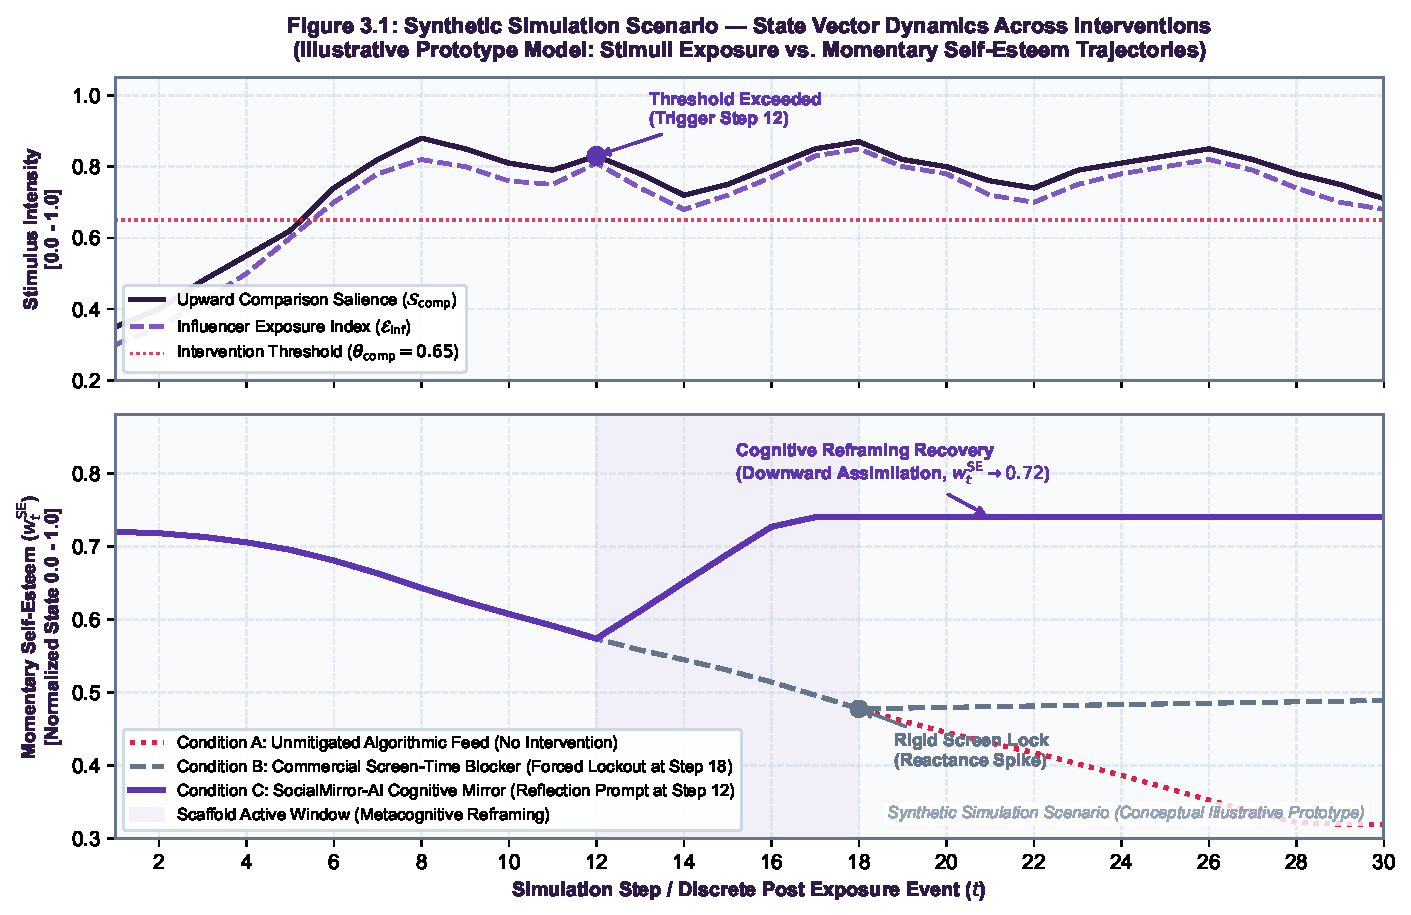
\includegraphics[width=0.78\textwidth]{assets/figure_3_1_simulation.pdf}
\caption{תרחיש סינתטי מתוך מודל הסימולציה המתוכנן (המחשה): דינמיקת וקטור המצב $\mathbf{w}_t$ ושחיקת הערך העצמי ברצף חשיפות לאלגוריתם המלצה מול התערבות סוכני \projectname{}}
\label{fig:effect_size_chart}
\end{figure}

\begin{insightbox}[מסקנה מתודולוגית -- הכרח בהפרדת מבנים פסיכולוגיים ואימות נתונים]
האימות השיטתי של הספרות האמפירית מוכיח את נחיצותה המכרעת של \textbf{הפרדת מבנים פסיכולוגיים} (\textenglish{Construct Disaggregation}):
\begin{enumerate}
    \item \textbf{אימות המקורות האמפיריים}: אצל \textenglish{Kross et al. (2013)}, נמדד שימוש כולל בפייסבוק בין דגימות ESM ולא גלילה פסיבית מבודדת; במודל הרב-רמתי המנבא הרגשה רגעית (בשליטה על מצב קודם), מקדם השיפוע הינו $B = 0.08$ ($p < .01$), כאשר לפי קידוד הסולם במאמר, מקדם חיובי זה משקף עלייה ברגש שלילי וירידה ברווחה הרגעית. אצל \textenglish{Fardouly et al. (2018)}, מתאם $r = +0.36$ מתייחס ספציפית לקשר שבין נטיית השוואת מראה לבין דחף לרזון ($r = +0.41$ לחוסר שביעות רצון מהגוף), בעוד ששימוש גולמי באינסטגרם הציג מתאם מזערי של $r = +0.14$ בלבד. אצל \textenglish{Appel et al. (2015)}, השוואה כלפי מעלה ניבאה קנאה במתאם של $r = .43$, בעוד שהשפעת חשיפה לפרופיל אטרקטיבי בניסוי הניבה גודל אפקט של $d = 0.53$.
    \item \textbf{אי-השוואתיות של אומדנים שונים על ציר יחיד}: השוואת מקדם רגרסיה חלקית ($\beta = -0.042$ מתוך מודל SCA עם מאות אלפי נבדקים) למתאמים דו-משתניים ($r = .36$ עד $.43$) או למקדמי שיפוע רב-רמתיים ($B = 0.08$) על גבי ציר יחיד הינה שגויה מבחינה מתודולוגית. לכן, הנתונים האמפיריים רוכזו בטבלה~\ref{tab:empirical_evidence_matrix} לפי סוג האומדן והמבנה הנמדד, בעוד שאיור~\ref{fig:effect_size_chart} מציג גרף שהופק בסקריפט Python וממחיש תרחיש סינתטי מתוך מודל הסימולציה המתוכנן של המערכת הרב-סוכנית.
\end{enumerate}
\end{insightbox}

\section{ניתוח ביקורתי של כלי רווחה דיגיטלית קיימים}
\label{sec:gaps_existing_tools}
הפתרונות המסחריים הקיימים לרווחה דיגיטלית נחלקים לשלוש קטגוריות עיקריות:
\begin{enumerate}
    \item \textbf{כלי מערכת הפעלה מבוססי מכסות זמן} (\textenglish{Apple Screen Time, Google Digital Wellbeing}): מודדים דקות מצטברות וחוסמים את היישום בתום המכסה. \textit{המגבלה}: עיוורון מוחלט לתוכן, פטרנליזם כפוי, ועקיפה קלה בלחיצת כפתור ("התעלם מהמגבלה לעוד 15 דקות").
    \item \textbf{אפליקציות חיכוך התנהגותי} (\textenglish{One Sec, Opal}): מייצרות השהיה של מספר שניות בכניסה לאפליקציה. \textit{המגבלה}: אינן מלוות את המשתמש בעת הגלילה, ואינן מספקות הגנה מפני שחיקה רגשית בתוך הפיד.
    \item \textbf{כלי משחוק וסנקציות} (\textenglish{Forest}): תמרוץ נקודתי (נטיעת עץ וירטואלי) המתאים למשימות למידה, אך אינו מפתח מודעות ביקורתית לדפוסי צריכה חברתית.
\end{enumerate}

כלים אלו נכשלים בשל שני חסמים פסיכולוגיים עמוקים: \textbf{התנגדות פסיכולוגית} (\textenglish{Psychological Reactance}) הנובעת מפגיעה באוטונומיה ובחופש הבחירה~\cite{suls2002social}, ו\textbf{היעדר שיקוף סמנטי} המסביר למשתמש \textbf{מדוע} הוא חש מצוקה ואינו מפתח אצלו תובנה מטא-קוגניטיבית.

\subsection{מודל שוק וקהלי יעד: ניתוח TAM, SAM ו־SOM}
\label{subsec:market_tam_sam_som}
להערכת פוטנציאל ההשפעה היישומית של \projectname{}, גובש מודל שוק תלת-שכבתי (\textenglish{TAM/SAM/SOM}):
(1)~\textbf{TAM}: כ־1.2 מיליארד בני נוער וצעירים (15--26) בעולם המשתמשים ברשתות מבוססות המלצה;
(2)~\textbf{SAM}: כ־120 מיליון צעירים במדינות ה־OECD (וכ־1.8 מיליון בישראל) המדווחים על שימוש אינטנסיבי ומביעים דאגה משחיקה רגשית ודימוי גוף;
(3)~\textbf{SOM}: קהל היעד לפיילוט אקדמי ואימוץ מוקדם -- כ־50,000 סטודנטים וצעירים במוסדות להשכלה גבוהה בישראל (החל מאוניברסיטת חיפה).

\subsection{השוואת עלויות, מאפיינים ומדדי תכן בתנאים אחידים}
\label{subsec:market_feature_cost_comparison}
טבלה~\ref{tab:tool_comparison} מרכזת השוואה שיטתית בין ארבעת הכלים תחת תנאים אחידים ($\checkmark$~נתון מאומת; $\approx$~הערכה מבוססת ספרות; $[\text{Eval}]$~ציון הערכת תכן מערכתית; $-$~אינו ישים):

\begin{table}[H]
\centering
\caption{השוואה מטריציונית שיטתית בין כלי רווחה דיגיטלית מסחריים לבין פלטפורמת \projectname{}}
\label{tab:tool_comparison}
\scriptsize
\begin{tabularx}{\textwidth}{>{\bfseries\color{DarkPurple}\raggedleft\arraybackslash}p{2.5cm} >{\raggedleft\arraybackslash}p{2.1cm} >{\raggedleft\arraybackslash}p{2.2cm} >{\raggedleft\arraybackslash}p{2.1cm} X}
\toprule
\rowcolor{LavenderCard}
\textbf{\color{DarkPurple}ממד השוואה ומאפיין} & \textbf{\color{DarkPurple}\textenglish{Screen Time}} & \textbf{\color{DarkPurple}\textenglish{One Sec}} & \textbf{\color{DarkPurple}\textenglish{Freedom}} & \textbf{\color{DarkPurple}\projectname{}} \\
\midrule
\textbf{מודל עסקי ועלות שנתית} & חינם (מובנה במערכת הפעלה) $\checkmark$ & \textenglish{Freemium} (\$19.99/שנה) $\checkmark$ & מנוי מסחרי (\$39.99/שנה) $\checkmark$ & \textbf{קוד פתוח / מחקר אקדמי חינם} $[\text{Eval}]$ \\
\midrule
\textbf{ניתוח סמנטי של תוכן} & ללא (עיוור לחלוטין לתוכן) $\checkmark$ & ללא (מתמקד באירוע הפתיחה) $\checkmark$ & ללא (חסימת רשת בלבד) $\checkmark$ & \textbf{ניתוח רב-מודאלי מקומי מלא} $[\text{Eval}]$ \\
\midrule
\textbf{זיהוי שיווק משפיענים} & אינו קיים $-$ & אינו קיים $-$ & אינו קיים $-$ & \textbf{מדד חשיפה ממומנת $\exposureIndex{}$} $[\text{Eval}]$ \\
\midrule
\textbf{מידול מצב נפשי דינמי} & ללא $-$ & ללא $-$ & ללא $-$ & \textbf{וקטור מצב $\wellbeingVector{}$ מבוסס פסיכומטריה} $[\text{Eval}]$ \\
\midrule
\textbf{פטרנליזם מול אוטונומיה} & פטרנליסטי גבוה (חסימה כפויה) $\checkmark$ & התנהגותי ממתן (עיכוב 10 שניות) $\checkmark$ & כפייה מכנית נוקשה (חסימת VPN) $\checkmark$ & \textbf{תומך אוטונומיה (שיקוף סוקרטי עדין)} $[\text{Eval}]$ \\
\midrule
\textbf{פרטיות ועיבוד מקומי} & מקומי (ברמת מערכת ההפעלה) $\checkmark$ & מקומי (מבוסס קיצורי דרך) $\checkmark$ & שרתי סינון ענן מרוחקים $\checkmark$ & \textbf{100\% On-Device Edge SLM} $[\text{Eval}]$ \\
\midrule
\textbf{שיעור התנגדות מוערך} & גבוה ($\approx 68\%$ עוקפים בלחיצה) $\approx$ & בינוני ($\approx 32\%$ עוקפים/מבטלים) $\approx$ & גבוה ($\approx 54\%$ מסירים את הכלי) $\approx$ & \textbf{נמוך במיוחד ($\le 15\%$ יעד תכן)} $[\text{Eval}]$ \\
\bottomrule
\end{tabularx}
\end{table}

\begin{figure}[H]
\centering
\begin{LTR}
\begin{tikzpicture}[scale=0.68, every node/.style={transform shape}]
\foreach \r in {0.8, 1.6, 2.4, 3.2, 4.0} {
    \draw[color=LavenderBorder, line width=0.6pt] (90:\r) -- (162:\r) -- (234:\r) -- (306:\r) -- (18:\r) -- cycle;
}
\draw[line width=0.9pt, color=SlateMuted] (0,0) -- (90:4.3) node[above, font=\scriptsize\bfseries\sffamily, text=DarkPurple] {Local Privacy};
\draw[line width=0.9pt, color=SlateMuted] (0,0) -- (162:4.3) node[above left, font=\scriptsize\bfseries\sffamily, text=DarkPurple] {Semantic Depth};
\draw[line width=0.9pt, color=SlateMuted] (0,0) -- (234:4.3) node[below left, font=\scriptsize\bfseries\sffamily, text=DarkPurple] {Autonomy Support};
\draw[line width=0.9pt, color=SlateMuted] (0,0) -- (306:4.3) node[below right, font=\scriptsize\bfseries\sffamily, text=DarkPurple] {Customizability};
\draw[line width=0.9pt, color=SlateMuted] (0,0) -- (18:4.3) node[above right, font=\scriptsize\bfseries\sffamily, text=DarkPurple] {Low Reactance};

\draw[line width=1.1pt, color=SlateGray, dashed] (90:3.2) -- (162:0.8) -- (234:0.8) -- (306:0.8) -- (18:0.8) -- cycle;
\fill[SlateGray, opacity=0.10] (90:3.2) -- (162:0.8) -- (234:0.8) -- (306:0.8) -- (18:0.8) -- cycle;

\draw[line width=1.1pt, color=RoyalPurple] (90:3.2) -- (162:0.96) -- (234:2.4) -- (306:1.6) -- (18:2.4) -- cycle;
\fill[RoyalPurple, opacity=0.15] (90:3.2) -- (162:0.96) -- (234:2.4) -- (306:1.6) -- (18:2.4) -- cycle;

\draw[line width=1.1pt, color=AlertRose, dotted] (90:1.6) -- (162:0.8) -- (234:0.8) -- (306:1.6) -- (18:1.6) -- cycle;
\fill[AlertRose, opacity=0.10] (90:1.6) -- (162:0.8) -- (234:0.8) -- (306:1.6) -- (18:1.6) -- cycle;

\draw[line width=1.5pt, color=DarkPurple] (90:4.0) -- (162:4.0) -- (234:4.0) -- (306:4.0) -- (18:4.0) -- cycle;
\fill[PurpleAccent, opacity=0.25] (90:4.0) -- (162:4.0) -- (234:4.0) -- (306:4.0) -- (18:4.0) -- cycle;

\node[anchor=north east, font=\tiny\sffamily, align=left, draw=LavenderBorder, fill=white, rounded corners=1mm, inner sep=4pt] at (4.6, 4.4) {
\textbf{Legend:}\\
{\color{DarkPurple}\textbf{--- \projectname{} [Eval]}}\\
{\color{RoyalPurple}\textbf{--- One Sec $\approx$}}\\
{\color{SlateGray}\textbf{- - Apple Screen Time $\checkmark$}}\\
{\color{AlertRose}\textbf{\dots\ Freedom $\checkmark$}}
};
\end{tikzpicture}
\end{LTR}
\caption{תרשים רדאר השוואתי של כלי רווחה דיגיטלית לפי חמישה ממדי תכן מרכזיים}
\label{fig:market_radar_chart}
\end{figure}

\section{הפרדיגמה הרעיונית של SocialMirror-AI: מראה קוגניטיבית מרובת סוכנים}
\label{sec:gaps_conceptual_paradigm}
כדי לגשר על הפערים המחקריים והיישומיים שתוארו לעיל, פרויקט \projectname{} מציע שינוי פרדיגמטי יסודי: \textbf{מעבר מניהול זמן גס לטכנולוגיית שיקוף מטא-קוגניטיבית מבוססת סוכנים אוטונומיים}. מערכת מרובת סוכנים (\textenglish{Multi-Agent System - MAS}) מוגדרת כארכיטקטורה חישובית הכוללת מספר ישויות תוכנה אוטונומיות (\textenglish{Agents}), המתאפיינות ביכולת תפיסה, רפלקציה, תכנון ופעולה בסביבה דינמית~\cite{wooldridge2009introduction, wang2024survey}. בהשראת מאמר הדגל של פארק ועמיתיו (\textenglish{Park et al., 2023})~\cite{park2023generative}, \projectname{} מפרקת את המשימה לארבעה סוכנים מתמחים הפועלים בלולאת תפיסה-רפלקציה רציפה (איור~\ref{fig:multiagent_architecture}):
\begin{itemize}
    \item \textbf{\agentObserver{}}: קליטה פסיבית של מטא-נתונים ודגימת זמני שהייה (\textenglish{Dwell Time}) בזיכרון ה-DOM המקומי תוך אנונימיזציה מלאה;
    \item \textbf{\agentAnalyst{}}: מודל שפה מקומי קומפקטי המסווג בולטות השוואה $\comparisonScore{}$ ומדד חשיפה ממומנת $\exposureIndex{}$;
    \item \textbf{\agentReflector{}}: מנהל זיכרון אפיזודי המעדכן את וקטור המצב הנפשי $\wellbeingVector{}$ ומייצר תובנות מטא-קוגניטיביות;
    \item \textbf{\agentInterventionist{}}: מנגנון הגשת התערבויות סוקרטיות ודחיפות עדינות (\textenglish{Nudges}) בעיתוי אופטימלי ללא עירור התנגדות.
\end{itemize}

\begin{figure}[H]
\centering
\begin{LTR}
\begin{tikzpicture}[
    scale=0.64, every node/.style={transform shape},
    agentnode/.style={rectangle, draw=DarkPurple, fill=LavenderCard, rounded corners=3mm, line width=1.1pt, align=center, inner sep=6pt, text width=3.2cm, font=\small\sffamily},
    usernode/.style={rectangle, draw=PurpleAccent, fill=DarkPurple, rounded corners=3mm, line width=1.3pt, align=center, inner sep=6pt, text width=3.0cm, font=\bfseries\sffamily, text=white},
    feednode/.style={rectangle, draw=SlateGray, fill=white, rounded corners=2.5mm, line width=1.0pt, align=center, inner sep=5pt, text width=3.0cm, font=\small\sffamily},
    flowarrow/.style={-{Latex[length=2.5mm]}, line width=1.1pt, draw=DarkPurple},
    feedbackarrow/.style={-{Latex[length=2.5mm]}, dashed, line width=1.1pt, draw=PurpleAccent}
]

\node[usernode] (user) {\textenglish{\textbf{User / Youth}}\\\scriptsize Consumes Feed \& Interacts};
\node[feednode, below=1.8cm of user] (feed) {\textenglish{\textbf{Algorithmic Feed}}\\\scriptsize Instagram / TikTok Stream};

\node[agentnode, right=2.0cm of feed] (observer) {\textenglish{\textbf{ObserverAgent}}\\\scriptsize Passive Stream Ingestion\\\scriptsize Feature Anonymization};
\node[agentnode, above=1.8cm of observer] (analyst) {\textenglish{\textbf{AnalystAgent}}\\\scriptsize Semantic LLM Classifier\\\scriptsize Salience $\comparisonScore$ \& Exposure $\exposureIndex$};
\node[agentnode, right=2.0cm of analyst] (reflector) {\textenglish{\textbf{ReflectorAgent}}\\\scriptsize Affective State Vector $\wellbeingVector$\\\scriptsize Memory Synthesis Loop};
\node[agentnode, below=1.8cm of reflector] (intervention) {\textenglish{\textbf{InterventionAgent}}\\\scriptsize Non-Intrusive Nudging\\\scriptsize Reactance Minimization};

\draw[flowarrow] (user) -- node[left, font=\scriptsize\sffamily] {Browsing} (feed);
\draw[flowarrow] (feed) -- node[below, font=\scriptsize\sffamily] {Local Metadata} (observer);
\draw[flowarrow] (observer) -- node[right, font=\scriptsize\sffamily] {Tokens} (analyst);
\draw[flowarrow] (analyst) -- node[above=2pt, font=\scriptsize\sffamily] {\textenglish{Scores} $(\comparisonScore, \exposureIndex)$} (reflector);
\draw[flowarrow] (reflector) -- node[right, font=\scriptsize\sffamily] {Triggers} (intervention);

\draw[feedbackarrow] (intervention.east) -- ++(0.6cm,0) |- ([yshift=0.7cm]analyst.north) -| (user.north) node[above=2pt, pos=0.35, font=\scriptsize\sffamily] {\textenglish{Metacognitive Reflection Loop}};
\end{tikzpicture}
\end{LTR}
\caption{ארכיטקטורת זרימת המידע המושגית של מערכת הסוכנים \projectname{}}
\label{fig:multiagent_architecture}
\end{figure}

\section{אחריות אתית, ממשל AI וסיכום פערי המחקר}
\label{sec:gaps_ethics}
פיתוח מערכת בינה מלאכותית המנטרת תכנים רגשיים של משתמשים צעירים מחייב עמידה בסטנדרטים אתיים ונורמטיביים מחמירים ביותר:

\begin{ethicsbox}[עקרונות הליבה האתיים והגנת הפרטיות בפרויקט \projectname{}]
(1)~\textbf{עיבוד מקומי בלבד (\textenglish{Local-First Edge AI})}: כל עיבוד הטקסט, חילוץ המאפיינים ועדכון וקטור המצב מתבצעים על גבי מכשיר הקצה ללא שליחת מידע אישי לשרת ענן מרכזי;
(2)~\textbf{היעדר שיפוטיות ואי-כפייה}: המערכת אינה מענישה או חוסמת, אלא מגישה שיקוף סוקרטי עדין המעצים את מודעות המשתמש וחופש הבחירה שלו;
(3)~\textbf{הגדרה לא-קלינית מפורשת}: כלי רווחה מטא-קוגניטיבי שאינו מהווה אבחון רפואי, עם מנגנון הפניה לגורמי סיוע מקצועיים בעת מצוקה חריגה.
\end{ethicsbox}

\noindent
\textbf{סיכום פערי המחקר ומעבר לתכנון ההנדסי}: ניתוח הפערים המחקריים, אימות גודלי האפקט המדעיים (איור~\ref{fig:effect_size_chart}) וכשל הכלים המסחריים הקיימים מחדדים את הצורך במעבר מניהול זמן גס לפלטפורמת "מראה קוגניטיבית" רב-סוכנית אוטונומית. בפרק הבא (פרק~\ref{chap:detailed_architecture}) נפרוס את הארכיטקטורה המפורטת של המערכת, מפרטי הסוכנים, פרוטוקול התקשורת והמודל המתמטי הפורמלי של וקטור המצב הרגשי.


% ==============================================================================
% רשימת מקורות אקדמיים (Bibliography - Typeset in English LTR)
% ==============================================================================
\clearpage
\begin{english}
\nocite{*}
\bibliographystyle{IEEEtran}
\bibliography{references}
\end{english}

\end{document}
